\documentclass[a4paper,12pt]{article}
\usepackage{amsmath}
\usepackage{listings}
\usepackage{xcolor}
\usepackage{float}
\usepackage{graphicx}
\usepackage{hyperref}
\usepackage{multicol}
\usepackage{enumitem}

\title{Into to Machine Learning - Sheet 3}
\author{Ibrahim Mohamed \\ ID: 7790}
\date{\today}

\begin{document}

\maketitle
\section*{Note}
This assignment was written using LaTeX. The source code for the document and the code used in this assignment can be found in the following GitHub link:
\url{https://github.com/H1MAA/Intro-To-Machine-Assignments}

\thispagestyle{empty}
\newpage

\section{Linear Regression}
\subsection{Question 1}
\textbf{Problem:} Find the least square regression line for the following set of data:
\[
\{(-1,0), (0,2), (1,4), (2,5)\}
\]

\textbf{Solution:}
\begin{enumerate}
    \item For Linear regression I will use the equation: 
\[
a = \frac{n(\sum xy) - (\sum x)(\sum y)}{n(\sum x^2) - (\sum x)^2}
\]
\[
b = \frac{1}{n}(\sum y - a\sum x)
\]
\item I defined the following equations in the function leastsquares in python:
\begin{figure}[H]
    \centering
    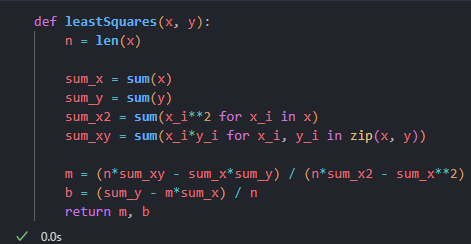
\includegraphics[width=0.7\textwidth]{leastSquaresFunction.png}
    \caption{Least Squares Function}
    \label{fig:least_squares_function}
\end{figure}
\begin{multicols}{2}
    \item when entering the data above i get: 
    \[
    a = 1.7, \quad b = 1.9
    \]
    The equation of the line is:
    \[
    y = 1.7x + 1.9
    \]
    \item The plot of the data and the line is shown to the right
    \begin{figure}[H]
        \centering
        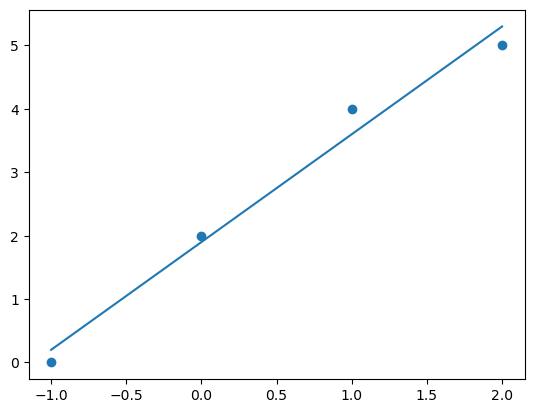
\includegraphics[width=0.4\textwidth]{leastSquaresOut.png}
        \caption{Least Squares Plot}
        \label{fig:least_squares_plot}
    \end{figure}
\end{multicols}
\end{enumerate}

\newpage
\subsection{Question 2}
\textbf{Problem:} 2. The value of x and their corresponding values of y are shown in the table below.

\begin{table}[H]
    \centering
    \begin{tabular}{|c|c|c|c|c|c|}
        \hline
        x & 0 & 1 & 2 & 3 & 4 \\
        \hline
        y & 2 & 3 & 5 & 4 & 6 \\
        \hline
    \end{tabular}
    \caption{Problem Givens}
    \label{tab:xy_values}
\end{table}

a) Find the least square regression line y = ax + b.\\

b) Estimate the value of y when x = 10.

\textbf{Solution:}
\begin{enumerate}
    \item Using the same function as in the previous question to find the least squares regression line for the data in the table above. The output of the function is shown below:
    \item the output of the function is:
    \[
    a = 0.9, b = 2.2
    \]
    The equation of the line is:
    \[
    y = 0.9x + 2.2
    \]
    \item The value of y given x = 10 is:
    \[
    y = 0.9(10) + 2.2 = 11.2
    \]
\end{enumerate}
\newpage

\subsection{Question 3}
\textbf{Problem:} 
Apply linear regression analytic form, use matrix inverse, to find the parameters of the best-fit line through the 6 points \(\{(2,2), (0,0), (-1,1), (1,-1), (-2,0), (2,0)\}\), shown in the figure below.

\textbf{Solution:}
\begin{enumerate}[label=\alph*)]
    \item
    \[
    \mathbf{w} = (\mathbf{X}^T \mathbf{X})^{-1} \mathbf{X}^T \mathbf{t}
    \]
    
    \[
    \mathbf{X} = \begin{bmatrix}
    1 & 2 \\
    1 & 0 \\
    1 & -1 \\
    1 & 1 \\
    1 & -2 \\
    1 & 2 \\
    \end{bmatrix}, \quad \mathbf{t} = \begin{bmatrix}
    2 \\
    0 \\
    1 \\
    -1 \\
    0 \\
    0 \\
    \end{bmatrix}
    \]

    \[
    (\mathbf{X}^T \mathbf{X})^{-1} = \left(\begin{bmatrix}
        1 & 1 & 1 & 1 & 1 & 1 \\
        2 & 0 & -1 & 1 & -2 & 2 \\
    \end{bmatrix} \begin{bmatrix}
        1 & 2 \\
        1 & 0 \\
        1 & -1 \\
        1 & 1 \\
        1 & -2 \\
        1 & 2 \\
    \end{bmatrix}\right)^{-1} = \begin{bmatrix}
        6 & 2 \\
        2 & 14 \\
    \end{bmatrix}^{-1}
    \]
    \[(\mathbf{X}^T \mathbf{X})^{-1} = \frac{1}{80} \begin{bmatrix}
        14 & -2 \\
        -2 & 6 \\
        \end{bmatrix} = \begin{bmatrix}
            0.175 & -0.025 \\
            -0.025 & 0.075 \\
        \end{bmatrix}   
    \]

    \[
    \quad \mathbf{X}^T \mathbf{t} = \begin{bmatrix}
        1 & 1 & 1 & 1 & 1 & 1 \\
        2 & 0 & -1 & 1 & -2 & 2 \\
    \end{bmatrix} \begin{bmatrix}
        2 \\
        0 \\
        1 \\
        -1 \\
        0 \\
        0 \\
    \end{bmatrix} = \begin{bmatrix}
    2 \\
    2 \\
    \end{bmatrix}
    \]
    
    \[
    \mathbf{w} = \begin{bmatrix}
    0.175 & -0.025 \\
    -0.025 & 0.075 \\
    \end{bmatrix} \begin{bmatrix}
    \end{bmatrix}
     \begin{bmatrix}
    2 \\
    2 \\
    \end{bmatrix} = \begin{bmatrix}
    0.3 \\
    0.1 \\
    \end{bmatrix}
    \]

    w = 0.1, b = 0.3, Therefore, the equation of the best-fit line is:
    \[
    y = 0.1x + 0.3
    \]

    \item The plot of the data points and the best-fit line is shown below:
    \begin{figure}[H]
        \centering
        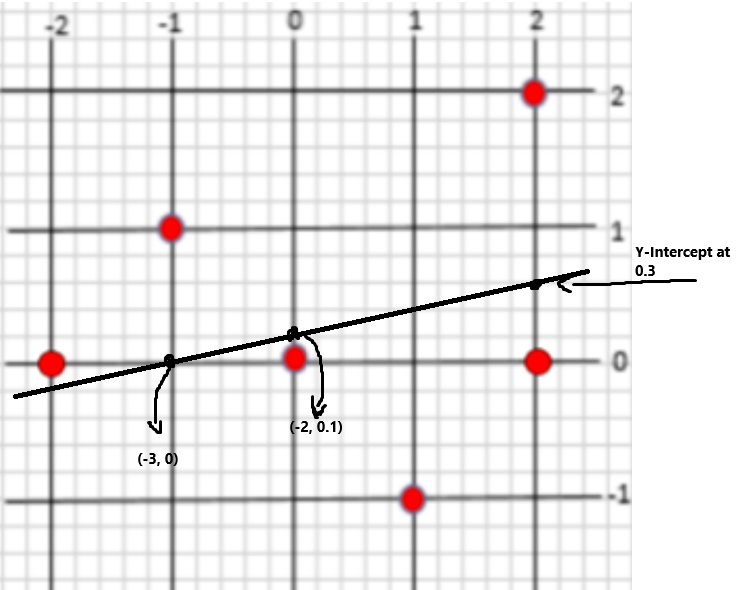
\includegraphics[width=0.8\textwidth]{bestFit.png}
        \caption{Best-Fit Line}
        \label{fig:best_fit_line}
    \end{figure}

    \item The sum of the squared loss is calculated as follows:
    \[
\text{Loss} = \sum_{i=1}^{n} (y_i - t)^2
\]
\[
\begin{array}{rcl}
    (2,2)   &\rightarrow& y = 0.5, \quad t = 2,  \quad\quad \text{Loss} = (2 - 0.5)^2 = 2.25 \\
    (0,0)   &\rightarrow& y = 0.3, \quad t = 0,  \quad\quad \text{Loss} = (0 - 0.3)^2 = 0.09 \\
    (-1,1)  &\rightarrow& y = 0.2, \quad t = 1,  \quad\quad \text{Loss} = (1 - 0.2)^2 = 0.64 \\
    (1,-1)  &\rightarrow& y = 0.4, \quad t = -1,      \quad \text{Loss} = (-1 - 0.4)^2 = 1.96 \\
    (-2,0)  &\rightarrow& y = 0.1, \quad t = 0,  \quad\quad \text{Loss} = (0 - 0.1)^2 = 0.01 \\
    (2,0)   &\rightarrow& y = 0.5, \quad t = 0,  \quad\quad \text{Loss} = (0 - 0.5)^2 = 0.25 \\
\end{array}
\]
\[
\sum_{i=1}^{n} (y_i -t)^2 = 2.25 + 0.09 + 0.64 + 1.96 + 0.01 + 0.25 = 5.2
\]

\newpage
    \item Linear regression is sensitive to noise. To illustrate this, we can remove the outlier and recalculate the best-fit line. The new data points are:
    \[
    \mathbf{X} = \begin{bmatrix}
    1 & 0 \\
    1 & -1 \\
    1 & 1 \\
    1 & -2 \\
    1 & 2 \\
    \end{bmatrix}, \quad \mathbf{y} = \begin{bmatrix}
    0 \\
    1 \\
    -1 \\
    0 \\
    0 \\
    \end{bmatrix}
    \]

    Recalculating $W = (X^T X)^{-1} X^T y$:
    \[
    W = \begin{bmatrix}
        5 & 0 \\
        0 & 10 \\
    \end{bmatrix}^{-1} \begin{bmatrix}
        0 \\
        -2
    \end{bmatrix} = \begin{bmatrix}
        0.2 & 0 \\
        0 & 0.1
    \end{bmatrix} \begin{bmatrix}
        0 \\
        -2
    \end{bmatrix} 
    \]
    \[
    W = \begin{bmatrix}
        0\\
        -0.2
    \end{bmatrix}, b = 0, w = -0.2, \\
    \quad \text{The new equation is:} \quad y = -0.2x
    \]

    Comparing this to the previous equation, we can calcuate loss:\\
    old line, y = 0.1x + 0.3, loss without outlier:

    \[
    \sum_{i=1}^{n} (y_i -t)^2 = 0.09 + 0.64 + 1.96 + 0.01 +0.25 = 2.95
    \]

    new line, y = -0.2x, loss:
    \[
    \begin{array}{rcl}
        (0,0)   &\rightarrow& y = 0.0,  \quad\quad t = 0,   \quad\quad \text{Loss} = (0 - 0)^2 = 0 \\
        (-1,1)  &\rightarrow& y = 0.2,  \quad\quad t = 1,   \quad\quad \text{Loss} = (1 - 0.2)^2 = 0.64 \\
        (1,-1)  &\rightarrow& y = -0.2, \quad t = -1,       \quad \text{Loss} = (-1 - (-0.2))^2 = 0.64 \\
        (-2,0)  &\rightarrow& y = 0.4,  \quad\quad t = 0,   \quad\quad \text{Loss} = (0 - 0.4)^2 = 0.16 \\
        (2,0)   &\rightarrow& y = -0.4, \quad t = 0,        \quad\quad \text{Loss} = (0 - (-0.4))^2 = 0.16 \\
    \end{array}
    \]
    \[
    \sum_{i=1}^{n} (y_i -t)^2 = 0 + 0.64 + 0.64 + 0.16 + 0.16 = 1.6
    \]

    as we can see, $1.6 < 2.95$, the loss is smaller without the outlier.
   
    \item Estimating \(y\) for \(x = -0.5\), \(x = 0.5\), and \(x = 1.5\):\\
    using old line, \(y = 0.1x + 0.3\):
    \[
    \begin{aligned}
        y_1 = 0.1(-0.5) + 0.3 &= 0.25, &y_2 = 0.1(0.5) + 0.3 &= 0.35
    \end{aligned}
    \]
    \[
    y_3 = 0.1(1.5) + 0.3 = 0.45
    \]

    using new line, \(y = -0.2x\):
    \[
    \begin{aligned}
        y_1 = -0.2(-0.5) &= 0.1, &y_2 = -0.2(0.5) &= -0.1
    \end{aligned}
    \]
    \[
    y_3 = -0.2(1.5) = -0.3
    \]
\end{enumerate}

\end{document}